\section{Results}

We illustrate the behaviour of the AMG preconditioner and the INVK
solver on GPUs  by showing the results obtained on a linear system
arisen from a groundwater modelling application developed at the
Juelich Supercomputing Centre (JSC)  dealing with numerical simulation
of the filtration of 3D incompressible single-phase flows through
anisotropic porous media. It is an elliptic equation with no flow
boundary conditions. The linear systems arises from the discretization
of the equation performed by a cell-centered finite colume scheme
(two-point flux approximation) on a Cartesian grid, with nonzero
entries distributed over seven diagonals. In these tests, we will
consider a homogeneous permeability tensor.  
Weak scalability tests are performed, using approximately 2 millions
equations per process. The total dimension ranges from 2 millions up
to 256 millions of equations. 
This application comes from the framework of the Horizon 2020 EoCoE
Project 

We ran experiments on the JURECA supercomputer at the Juelich
Supercomputing Centre (JSC).  Each GPU compute node consists of two
NVIDIA Tesla K80 GPUs with a dual-GPU design, for a total of four
available GPU devices per compute nodes.  
We used PSBLAS 3.5 (combined with its extension plugin for extended
matrix formats and GPU plugin) and MLD2P4 2.1 (combined with AINV
plugin),  compiled with  GNU compilers (C and Fortran) version 5.4.0,
MVAPICH2 version 2.3 and with CUDA 8.0.61. 

Linear systems are solved using Conjugated Gradient (CG) and the
stopping criterion is based on the ratio bewteen 2-norms of the
residual and the right-hand side vector (when smaller than
$10^{-6}$). CG is use in conjuction with a V-cycle preconditioner. We
consider two different configurations. In the first case the V-cycle
preconditioner applies 1 pre and post sweep of Block Jacobi smoother
with INVK (approximate inverse based on the inversion of triangular
factors based on a positional drop strategy) as a solver. In the
second configuration it applies 2 per and post sweeps of Jacobi
solver. In both cases, we use 10 sweeps of Block Jacobi with INVK  as
coarsest level solver.   
For each configuration, we ran tests only on CPUs (with matrices in
CSR format) and using CPUs+GPUs (with matrices in ELG format). This
allows us to quantify the gain in efficiency in using GPUs.   

In tables \ref{cpu-invk} and \ref{gpu-invk} we show results for the case using BJAC(INVK) smoother on the inner levels.


\begin{table}[h!]
\centering
\caption{Numerical results for CG + ML preconditioner, runs on CPUs, with 1 sweep of BJAC(INVK) as smoother on inner levels.}
\label{cpu-invk}

\begin{tabular}{rrrrrrr}
% \multicolumn{1}{l}{np} & \multicolumn{1}{l}{levels} &   \multicolumn{1}{l}{Iters} & \multicolumn{1}{l}{\begin{tabular}[c]{@{}l@{}}Prec    \\  
%  time (s)\end{tabular}} &
%                           \multicolumn{1}{l}{\begin{tabular}[c]{@{}l@{}}Solve  \\  
% Time (s)\end{tabular}} &
%                          \multicolumn{1}{l}{\begin{tabular}[c]{@{}l@{}}Time per \\ 
% Iteration (ms)\end{tabular}} & \multicolumn{1}{l}{\begin{tabular}[c]{@{}l@{}}Total  \\   Time (s)\end{tabular}} \\ \hline
NP  & Levels & Iters & Tsetup & Tsolve & T/iter & Ttotal \\
    &        &       & (s)    & (s)    & (ms)   & (s)    \\
\hline
1   & 4       & 14  & 17.74 & 4.42  & 320      & 22.15   \\
2   & 4       & 15  & 19.43 & 5.05  & 340      & 24.47   \\
4   & 4       & 18  & 21.85 & 6.96  & 390      & 28.81   \\
8   & 4       & 20  & 28.32 & 8.05  & 400      & 36.37   \\
16  & 4       & 24  & 26.38 & 9.59  & 400      & 35.98   \\
32  & 4       & 29  & 23.52 & 11.42 & 390      & 34.93   \\
64  & 4       & 34  & 29.61 & 14.21 & 420      & 43.82   \\
128 & 5       & 29  & 28.39 & 13.19 & 450      & 41.58    \\
\hline
\end{tabular}
\end{table}

\begin{table}[h!]
\centering
\caption{Numerical results for CG + ML preconditioner, runs on GPUs, with 1 sweep of BJAC(INVK) as smoother on inner levels.}
\label{gpu-invk}

\begin{tabular}{rrrrrrrr}
% \multicolumn{1}{l}{np} & \multicolumn{1}{l}{levels} & \multicolumn{1}{l}{It} & \multicolumn{1}{l}{\begin{tabular}[c]{@{}l@{}}Prec    \\   time (s)\end{tabular}} & \multicolumn{1}{l}{\begin{tabular}[c]{@{}l@{}}Solve  \\  Time (s)\end{tabular}} & \multicolumn{1}{l}{\begin{tabular}[c]{@{}l@{}}Time per \\ Iteration (ms)\end{tabular}} & \multicolumn{1}{l}{\begin{tabular}[c]{@{}l@{}}Total  \\   Time (s)\end{tabular}} & \multicolumn{1}{l}{\begin{tabular}[c]{@{}l@{}}Speed up\\ cpu/gpu\end{tabular}} \\ \hline
NP  & Levels & Iters & Tsetup & Tsolve & T/iter & Ttotal & Speedup\\
    &        &       & (s)    & (s)    & (ms)   & (s)   &  \\
\hline
1   & 4       & 14  & 18.80 & 0.45 & 30   & 19.24& 9.92  \\
2   & 4       & 15  & 20.55 & 0.54 & 40   & 21.09& 9.40  \\
4   & 4       & 18  & 22.84 & 0.69 & 40   & 23.54& 10.08 \\
8   & 4       & 20  & 29.18 & 0.86 & 40   & 30.03& 9.40  \\
16  & 4       & 24  & 27.38 & 1.12 & 50   & 28.50& 8.57  \\
32  & 4       & 29  & 23.74 & 1.29 & 40   & 25.02& 8.85  \\
64  & 4       & 34  & 30.53 & 1.79 & 50   & 32.32& 7.94  \\
128 & 5       & 29  & 29.48 & 2.22 & 80   & 31.70& 5.94  \\
\hline
\end{tabular}
\end{table}




The results for the case using two sweeps of a Jacobi smoother on inner levels are shown in tables \ref{cpu-jac} and \ref{gpu-jac}

\begin{table}[h!]
\centering
\caption{Numerical results for CG + ML preconditioner, runs on CPUs, with 2 sweeps of JACOBI as smoother on inner levels.}
\label{cpu-jac}

\begin{tabular}{rrrrrrr}
% \multicolumn{1}{l}{np} & \multicolumn{1}{l}{levels} & \multicolumn{1}{l}{It} & \multicolumn{1}{l}{\begin{tabular}[c]{@{}l@{}}Prec    \\   time (s)\end{tabular}} & \multicolumn{1}{l}{\begin{tabular}[c]{@{}l@{}}Solve  \\  Time (s)\end{tabular}} & \multicolumn{1}{l}{\begin{tabular}[c]{@{}l@{}}Time per \\ Iteration (s)\end{tabular}} & \multicolumn{1}{l}{\begin{tabular}[c]{@{}l@{}}Total  \\   Time (s)\end{tabular}} \\ \hline
NP  & Levels & Iters & Tsetup & Tsolve & T/iter & Ttotal \\
    &        &       & (s)    & (s)    & (ms)   & (s)    \\
\hline
1   & 4       & 19  & 2.83  & 3.76  & 200   & 6.59    \\
2   & 4       & 21  & 3.65  & 4.57  & 220   & 8.23    \\
4   & 4       & 20  & 4.21  & 5.13  & 260   & 9.35    \\
8   & 4       & 25  & 4.75  & 6.58  & 260   & 11.33   \\
16  & 4       & 27  & 4.97  & 7.21  & 270   & 12.18   \\
32  & 4       & 31  & 4.88  & 8.21  & 260   & 13.09   \\
64  & 4       & 37  & 5.79  & 10.20 & 280   & 16.00   \\
128 & 5       & 31  & 6.72  & 11.16 & 360   & 17.88  \\
\hline
\end{tabular}
\end{table}

\begin{table}[h!]
\centering
\caption{Numerical results for CG + ML preconditioner, runs on GPUs, with 2 sweeps of JACOBI as smoother on inner levels.}
\label{gpu-jac}
\begin{tabular}{rrrrrrrr}
% \multicolumn{1}{l}{np} & \multicolumn{1}{l}{levels} & \multicolumn{1}{l}{It} & \multicolumn{1}{l}{\begin{tabular}[c]{@{}l@{}}Prec    \\   time (s)\end{tabular}} & \multicolumn{1}{l}{\begin{tabular}[c]{@{}l@{}}Solve  \\  Time (s)\end{tabular}} & \multicolumn{1}{l}{\begin{tabular}[c]{@{}l@{}}Time per \\ Iteration (s)\end{tabular}} & \multicolumn{1}{l}{\begin{tabular}[c]{@{}l@{}}Total  \\   Time (s)\end{tabular}} & \multicolumn{1}{l}{\begin{tabular}[c]{@{}l@{}}Speed up\\ cpu/gpu\end{tabular}} \\ \hline
NP  & Levels & Iters & Tsetup & Tsolve & T/iter & Ttotal & Speedup\\
    &        &       & (s)    & (s)    & (ms)   & (s)   &  \\
\hline
1   & 4       & 19  & 3.13  & 0.40 & 20   & 3.53 & 9.39  \\
2   & 4       & 21  & 4.06  & 0.52 & 20   & 4.59 & 8.73  \\
4   & 4       & 20  & 4.65  & 0.63 & 30   & 5.28 & 8.16  \\
8   & 4       & 25  & 5.20  & 0.85 & 30   & 6.05 & 7.74  \\
16  & 4       & 27  & 5.39  & 1.02 & 40   & 6.42 & 7.06  \\
32  & 4       & 31  & 5.35  & 1.24 & 40   & 6.59 & 6.61  \\
64  & 4       & 37  & 6.25  & 1.71 & 50   & 7.96 & 5.98  \\ 
128 & 5       & 31  & 7.19  & 2.23 & 70   & 9.43 & 5.00  \\
\hline
\end{tabular}
\end{table}


When GPUs are used, the last column shows the speed-up of the solver
phase on the gpu with respect to the cpu solve time. The speed-up
achieves a maximum value of 10 in the case of 8 processes and it
achieves a value slightly bigger than 5 with 128 processes. In this
latter case, the increasing number of levels leads to a decreasing in
the size of the coarsest level matrix, which can explain the
decreasing of the speed-up. Despite that, in all cases the use of GPUs
positively affects the performance of the solve phase.  
We point out that the all the cases examined show good algorithmic
scalability. It means that the number of iterations needed to achieve
convergence stays almost constant as the number of processes grows.  
Finally, we show that excellent scalability is achieved for the solve
phase, by plotting the time per single iteration versus the number of
processes (Figure \ref{fig:time_per_it}). In the case with GPUs, this
value is almost constant up to 64 processes. A small increasing can be
appreciated in the case with 128 process but, as previously pointed
out, this is due to the increasing in the number of levels and hence
in the complexity of the preconditioner.      

\begin{figure}[h!]
\caption{Time per iteration}
\centering
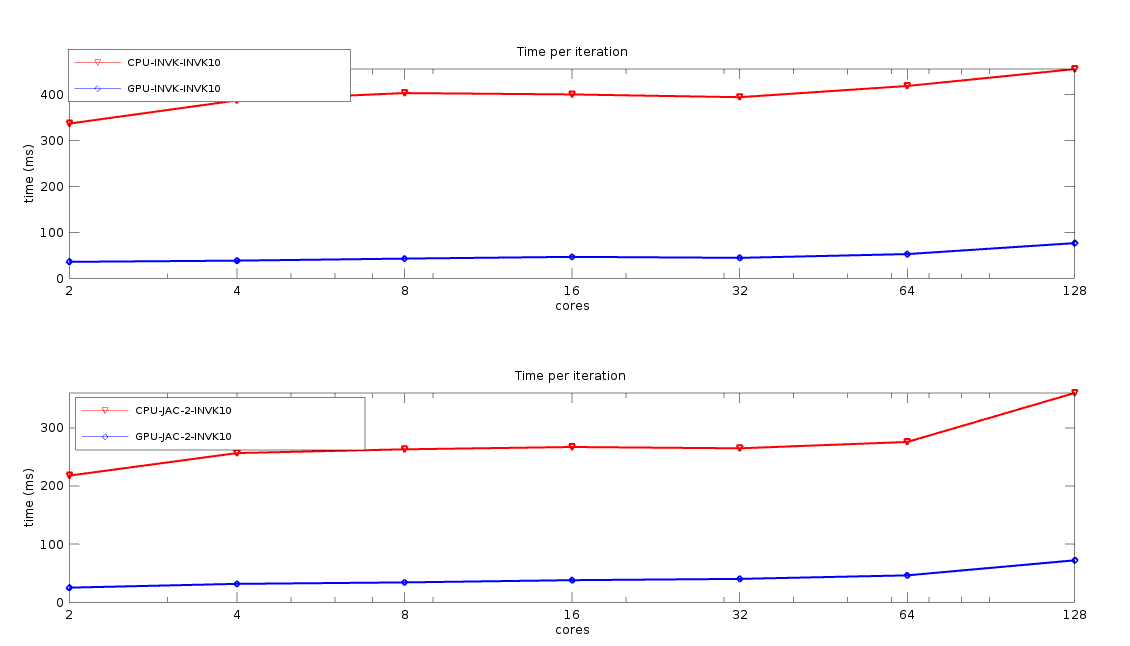
\includegraphics[width=1\textwidth]{time_per_it.png}
\label{fig:time_per_it}
\end{figure}


\begin{figure}
\begin{center}
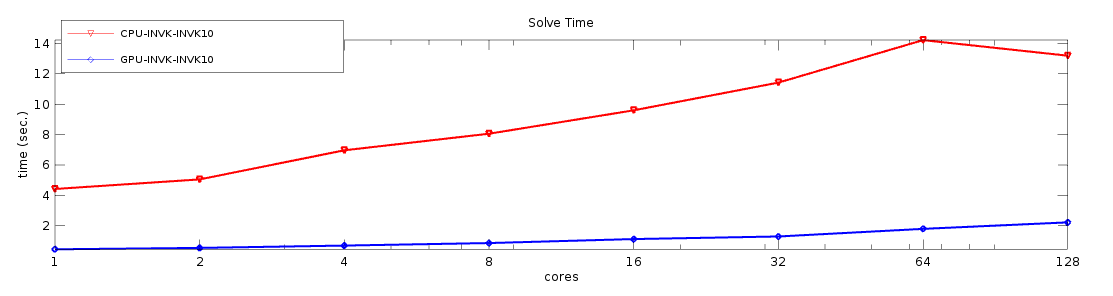
\includegraphics[width=.9\textwidth]{graf_invk.png}
\end{center}
\caption{INVK-INVK}
\end{figure}

\begin{figure}
\begin{center}
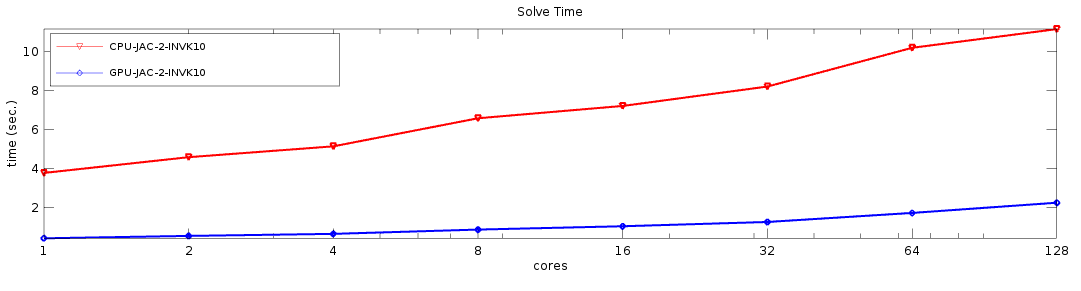
\includegraphics[width=.9\textwidth]{graf_jac2.png}
\end{center}
\caption{JAC2-INVK}
\end{figure}
